\chapter{Формальная постановка задач}
\label{cha:Formal}

\section{Общие обозначения и входной формат}
 Задача паллетизации представляет собой целое семейство задач на укладку паллет. 

 Фактически задача сводится к укладке прямоугольных коробок на прямоугольный поддон (палетту). 

 

Дана паллета с известным размером $W\times L$ и набор $S$ $K$ коробок с заданными размерами $S=\{s_1,s_2, ... s_K\}=\{(w_1,l_1,h_1),(w_2,l_2,h_2), ... (w_K,l_K,h_K)\}$. 

В качестве дополнительных параметров коробок могут использоваться масса коробок $m_k$ и "цвет" $c_k$.

%На первом этапе считаем, что высота всех коробок одинакова:

%$$h_1=h_2=...+h_K$$

Исходный массив имеет вид

\{SKU,Quantity,Length,Width,Height,Weight,Strength,Aisle,Caustic\}

Здесь 
\begin{itemize}
\item SKU - код позиции товара,
\item Quantity - количество коробок данного типа,
\item Length - длина коробки в мм,
\item Width - ширина коробки в мм,
\item Height - высота коробки в мм,
\item Weight - вес коробки в мм,
\item Strength - прочность коробки (не используется),
\item Aisle - тип содержимого (соответствует color в нашей постановке),
\item Caustic - "цвет", который в рамках текущей работы не используется
\end{itemize}

  
Необходимо выполнить укладку коробок на паллету  с выполнением ряда требований.

Каждый упакованный блок характеризуется двумя координатами: $<x_1,y_1,z_1>$ и $<x_2,y_2,z_2>$, где первыми записаны координаты нижнего левого угла (наиболее близкого к началу координат $<0,0,0>$), а вторыми – координаты с наибольшими значениями. Таким образом, решение задачи имеет вид $S={s_i=(<x_1^i,y_1^i,z_1^i>, <x_2^i,y_2^i,z_2^i>) | i=1,2,…,K}$.

Результат описывается в виде массива данных:

\begin{verbatim}
H_total Percolation W_total
SKU_i  x_1^i y_1^i z_1^i   x_2^i y_2^i ,z_2^i Aisle Weight
...

\end{verbatim}

Здесь:

$H_{total}$ - полная высота паллеты с коробками;

$Percolation= {(\sum_{i=1}^K w_i)}/{(W\times L \times H})$ - плотность упаковки (принимает значение от 0 до 1);

$W_{total}$ - полный  вес паллеты;

$SKU_i$ - код коробки во входном массиве;

$x_1^i,y_1^i,z_1^i$ - координаты угла $O_i$;

$x_2^i,y_2^i,z_2^i$ - координаты угла, противоположного $O_i$. 



Порядок следования записей должен соответствовать последовательности укладки коробок в паллету.

\begin{figure}[ht]
 
\center{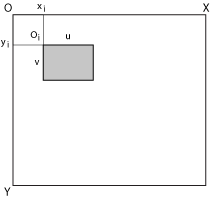
\includegraphics[width=250pt]{figures/T_4-1.png}} ) 
 
\caption{Описание укладки}
\label{ris:T_1-1}
\end{figure}
\paragraph{Пример входного и выходного  файла}

Входной файл COS-TEST-1-in.txt:
\begin{verbatim}
1
SKU,Quantity,Length,Width,Height,Weight,Strength,Aisle,Caustic
900001,6,600,400,200,12000,4,1,0,
900002,5,200,400,200,5000,4,2,0, 
\end{verbatim}

Выходной файл COS-TEST-1-out.txt:
\begin{verbatim}
2
400 1.00 97000
SKU_i,x_1^i,y_1^i,z_1^i,x_2^i,y_2^i,z_2^i,Aisle,Weight
900001,0,0,0,600,400,200,1,12000,
900001,800,0,0,1200,600,200,1,12000,
900002,600,0,0,800,400,200,2,5000,
900002,0,400,0,200,800,200,2,5000,
900002,200,400,0,400,800,200,2,5000,
900002,400,400,0,600,800,200,2,5000,
900002,800,600,0,1200,800,200,2,5000,
900001,0,0,200,600,400,400,1,12000,
900001,600,0,200,1200,400,400,1,12000,
900001,0,400,200,600,800,400,1,12000,
900001,600,400,200,1200,800,400,1,12000,
\end{verbatim}

В первой строке код паллеты из датасета.

Во второй строке 

400 1.00 97000

высота паллеты в мм, плотность укладки, общий вес в граммах.

Можно дополнить временем вычисления на референтном процессоре. 

\section{Распределение коробок между несколькими  паллетами адресной доставки}


Для каждого адреса $a$ известен  фиксированный  набор паллет
        $\mathcal{B}_a=\{P_{a,1},\dots,P_{a,N_a}\}$  
        одинакового основания $W\times L$, в каждом из которых находится список коробок, связанных с ними.

 
 Каждую коробку $s_k$, находящуюся в списках $P_{a_k,j}\in\mathcal{B}_{a_k}$ поместить строго на одну из паллет $P_{a_k,j}\in\mathcal{B}_{a_k}$.
 Соблюсти для каждой паллеты все геометрические.
  При этом необходимо стремиться к равномерной загрузке паллет одного адреса:
        \begin{itemize}
           \item минимизировать разброс по итоговым высотам паллет;
           \item повысить $Percolation$ в пределах заданного множества паллет.
        \end{itemize}
 

 
Входные и выходные данные должны быть в том же формате, что и для Задачи 1.  
Если в результате формируется   несколько паллет, то их содержимое выводится последовательно отдельными файлами.  